\documentclass[aspectratio=169]{beamer}
\usetheme{metropolis}         
\usecolortheme{default}
\usepackage{amsmath, amssymb}
\usepackage{graphicx}
\usepackage{booktabs}


% ---- Title info ----
\title{Discovering Context Effects from Raw Choice Data}
\subtitle{}
\author{}
\institute{}
\date{August 17, 2026}
\begin{document}

\begin{frame}
    \titlepage
\end{frame}

\begin{frame}{ choice example}
    \textbf{Setting:} IIT Madras $\rightarrow$ Airport

    \vspace{1em}

    Four real options:
    \begin{itemize}
        \item Car, Taxi, Bike, Bus
    \end{itemize}

    \vspace{0.5em}

    Natural preference:
    \begin{center}
        Car $\succ$ Taxi $\succ$ Bike $\succ$ Bus
    \end{center}

    \vspace{1em}

    \textit{Now what if we add walking?} \pause \hfill (takes 3 hours!)
\end{frame}
\begin{frame}{Independence of Irrelevant Alternatives}
    Walking should not change how we feel about Car vs Taxi.

    \vspace{0.5em}

    Formally, for any two sets $A, B$ and items $x, y$:
    \begin{equation*}
        \frac{P(x \mid A)}{P(y \mid A)} = \frac{P(x \mid B)}{P(y \mid B)}
    \end{equation*}

    \vspace{0.5em}

    Quick check with weights $w = (0.40, 0.25, 0.15, 0.12, 0.08)$:
    \begin{itemize}
        \item $A = \{C, T, Bi\}$, $B = \{C, T, W\}$
        \item $\frac{0.40}{0.25} = \frac{0.40}{0.25} \;\; \Rightarrow \;\; 1 = 1 \;\; \checkmark$
    \end{itemize}
\end{frame}
\begin{frame}{Multinomial logit | Bradley Terry Model}
    \begin{equation*}
        P(x \mid C) = \frac{\exp(v(x))}{\sum_{y \in C} \exp(v(y))}
    \end{equation*}

    \vspace{0.5em}

    Identifiability constraint (shift-invariance):
    \begin{equation*}
        \sum_y v(y) = 0
    \end{equation*}

    \vspace{0.5em}

    Example: $v(C) = 2.5, v(T) = -0.9$ gives the same $P$ as
    $v(C) = 1.7, v(T) = -1.7$.

    \vspace{0.3em}

    $\rightarrow$ centering makes the parameters unique.
\end{frame}

% ============================================================
% SLIDE 5 — IIA violations
% ============================================================
\begin{frame}{Violation of IIA}
    Experiments show that adding an option shifts the perceived
    attractiveness of existing ones.

    \vspace{1em}

    Classic examples:
    \begin{itemize}
        \item Decoy effect
        \item Similarity effect
        \item Compromise effect
    \end{itemize}

    \vspace{1em}

    $\rightarrow$ MNL cannot capture this.

    \vspace{0.3em}
    \small
    \textit{Seshadri, Peysakhovich, Ugander (ICML 2019).}
\end{frame}

% ============================================================
% SLIDE 6 — Universal logit
% ============================================================
\begin{frame}{Universal logit model}
    Idea: let the utility \emph{depend on the choice set}.

    \begin{equation*}
        P(x \mid C) = \frac{\exp(u(x \mid C))}{\sum_{y \in C} \exp(u(y \mid C))}
    \end{equation*}

    \vspace{0.5em}

    Constraint per set:
    \begin{equation*}
        \sum_{y \in C} u(y \mid C) = 0 \quad \forall\, C \subseteq \mathcal{X}
    \end{equation*}

    \vspace{0.5em}

    $\rightarrow$ this is expressive but parameter-heavy.
\end{frame}

% ============================================================
% SLIDE 7 — Lemma 1 + counting
% ============================================================
\begin{frame}{Lemma 1 (Seshadri, 2019)}
    Every $u(x \mid C)$ decomposes over subsets:
    \begin{equation*}
        u(x \mid C) = v(x) + \sum_{y} v(x \mid \{y\})
        + \sum_{\{y,z\}} v(x \mid \{y,z\}) + \dots
    \end{equation*}

    with $\sum_{x \notin B} v(x \mid B) = 0$ for every $B$.

    \vspace{1em}

    Worked count for $A = \{C, T, Bi\}$:
    \begin{center}
        9 raw parameters $-$ 4 constraints $=$ \fbox{5 free parameters}
    \end{center}
\end{frame}

% ============================================================
% SLIDE 8 — MLE setup
% ============================================================
\begin{frame}{Estimating parameters via MLE}
    Start with the pairwise case (Bradley-Terry).

    \vspace{0.5em}

    Log-likelihood over $N$ comparisons:
    \begin{equation*}
        \ell(\mathbf{v}) = \sum_{n=1}^{N} \log \sigma(v_{i_n} - v_{j_n})
    \end{equation*}

    Gradient has a very clean form:
    \begin{equation*}
        \frac{\partial \ell}{\partial v_k} = W_k - E_k
    \end{equation*}
    \vspace{0.3em}
    \textit{observed wins} $-$ \textit{expected wins} \\
    $\rightarrow$ moment matching at the MLE.
\end{frame}

\begin{frame}{Does it work? A quick empirical check}
    Setup:
    \begin{itemize}
        \item 5 items, weights from earlier
        \item $N = 2000$ simulated pairwise comparisons
        \item Fit two ways: I-LSR (\texttt{choix}) and GD from scratch
    \end{itemize}

    \vspace{0.3em}

    \begin{center}
        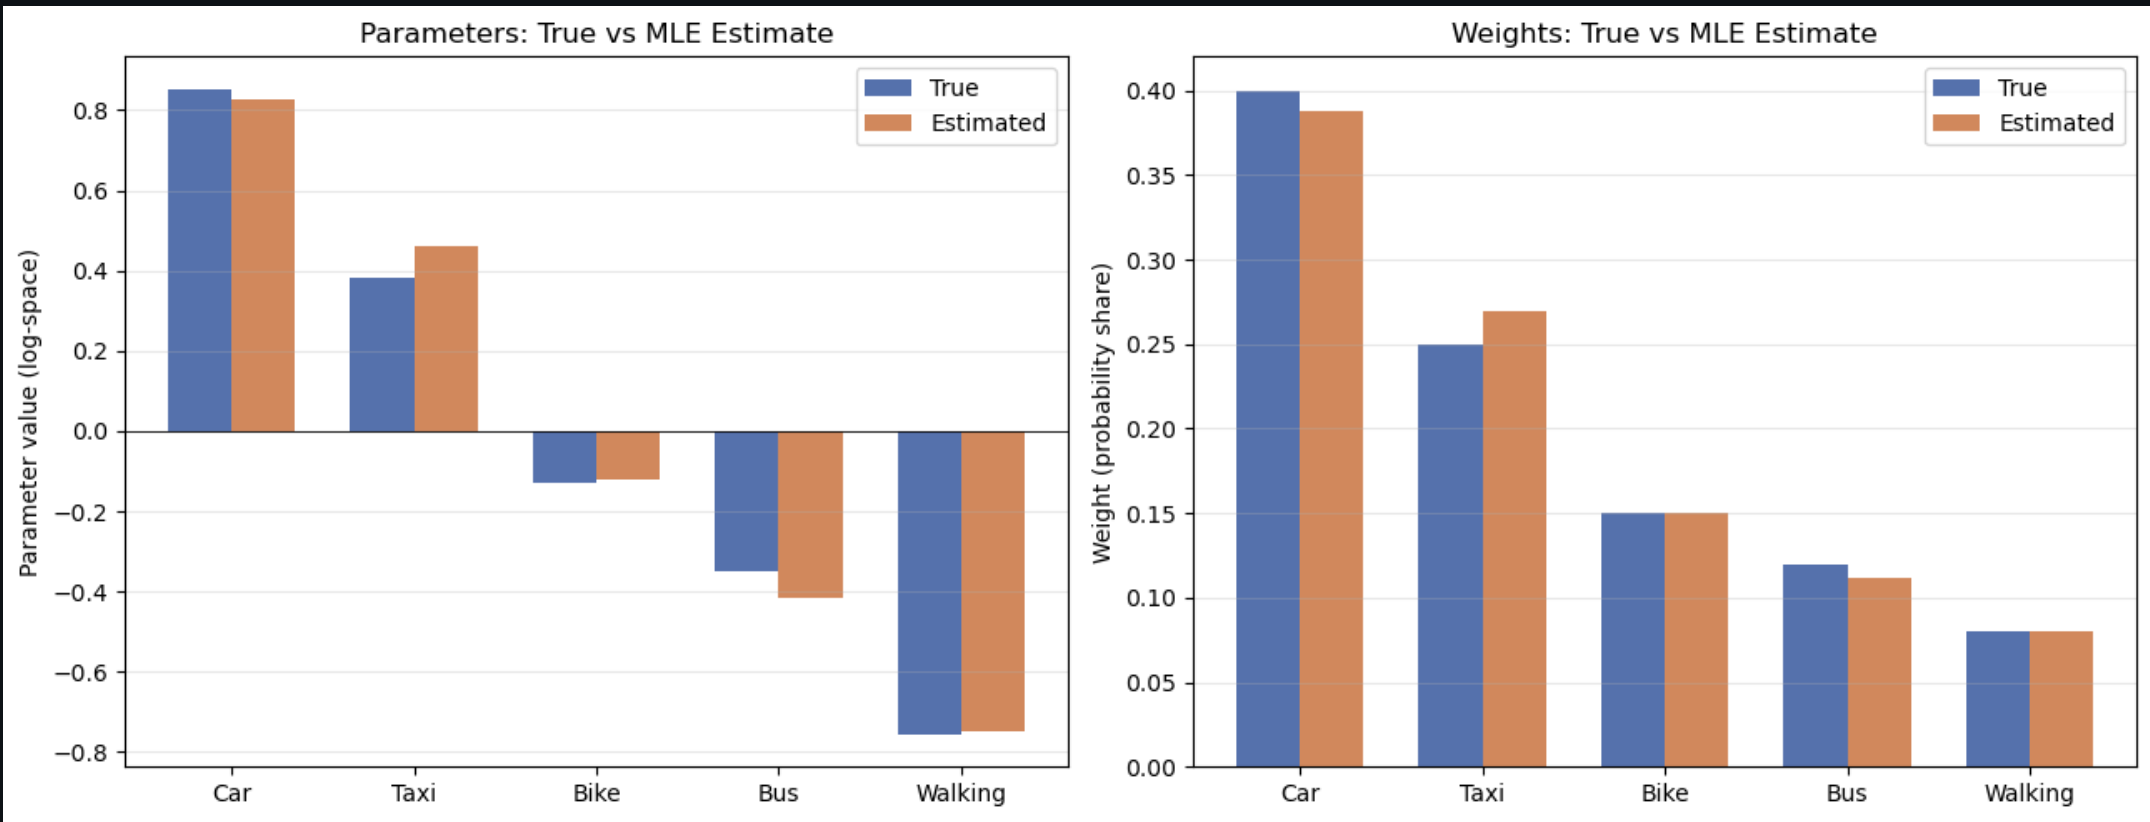
\includegraphics[width=0.85\linewidth]{mle_comparison.png}
    \end{center}

    \vspace{0.2em}
    Both methods recover the truth with MAE $\approx 0.04$.
\end{frame}
\begin{frame}{Next week..}
    \begin{itemize}
        \item Extend MLE to the context-dependent model (CDM) and low-rank CDMs
        \item Compare CDM vs MNL on IIA-violating data..
        \item And also understand and try to implement Tomlinson & Benson, KDD 2021, Learning Interpretable Feature Context Effects in Discrete Choice as its main goal is to discover how the features of the other available options change someone's choice... which is a different kind of structure than the low rank CDMs
    \end{itemize}

    \vspace{2em}

    \begin{center}
        \Large Thank you. 
    \end{center}
\end{frame}

\end{document}